\vspace{0.2in}
\section{Evaluation}
\label{sec-evaluation}

\begin{figure*}[t]
\begin{center}
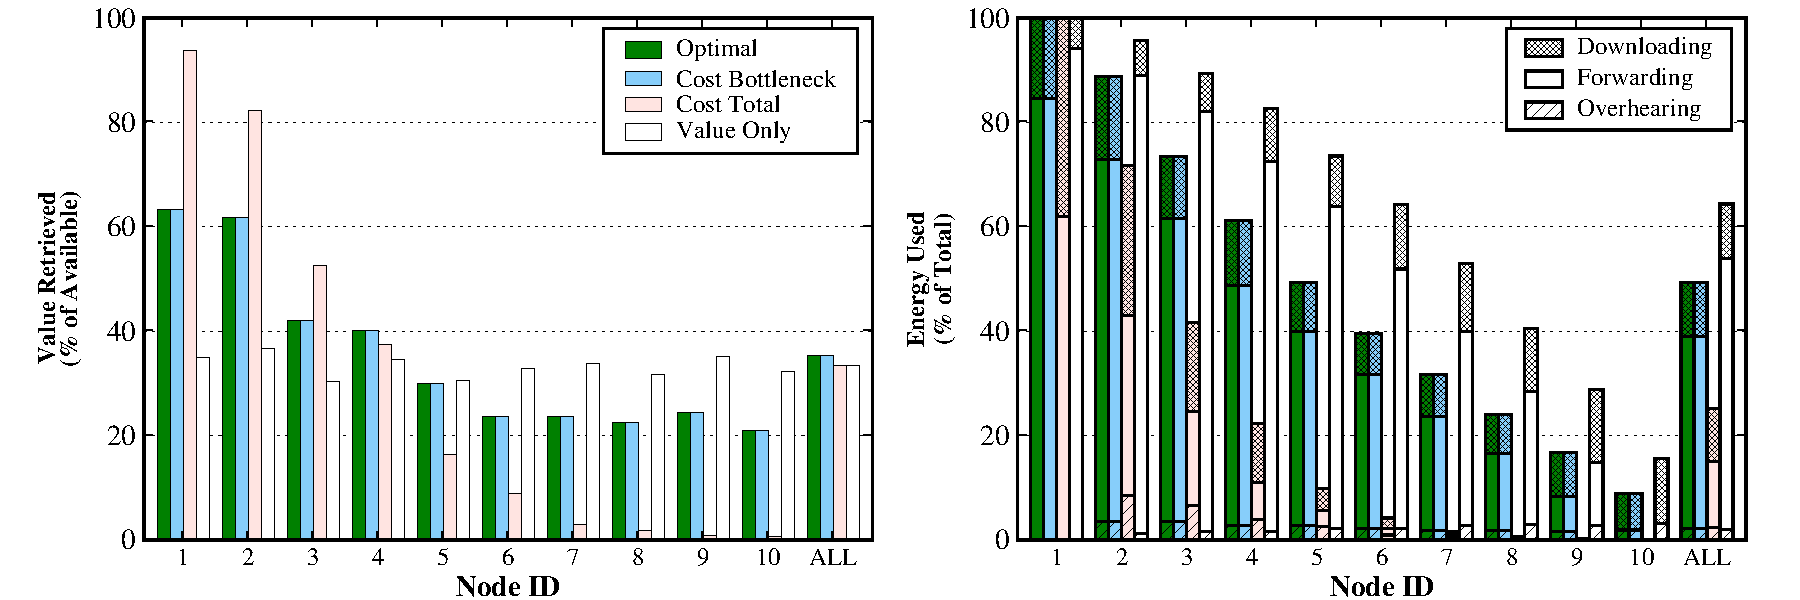
\includegraphics[width=1.0\hsize]{./figs/gwa/linear/BOTH.pdf}
\end{center}
\caption{\small {\bf Per-node distribution of ADU value and energy
usage for the linear simulation experiment.} 
{\em The top graph shows the amount of
data value downloaded from each node, while the bottom graph breaks down the
amount of energy used by each node into the downloading, routing and
overhearing components. Node~1 is closest to the base station.}}
\label{sec-eval-figlinear}
\end{figure*}

\begin{figure}[t]
\begin{center}
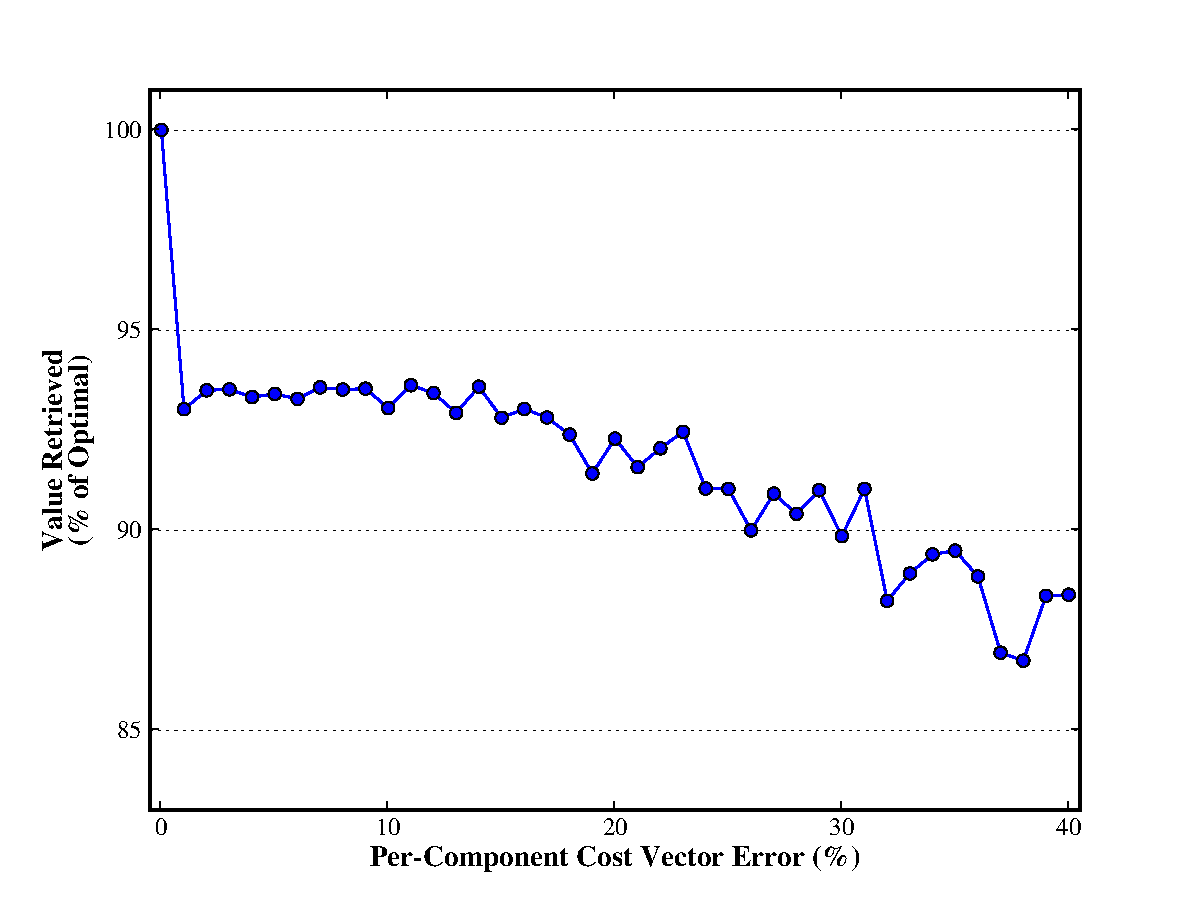
\includegraphics[width=1.0\hsize]{./figs/gwa/error/ERROR.pdf}
\end{center}
\caption{\small {\bf Effect of cost vector error on optimality.} 
{\em The
optimization process is guided by the cost vectors, but predicting the energy
cost of operations before they are performed can be difficult.  Here we show
the impact of introducing a degree of error into the cost vectors used by the
optimizer.  As can be seen, we can tolerate a relatively high degree of
error, as long as the shape of the cost vector does not change.}}
\label{sec-eval-figerror}
\end{figure}

This section presents a careful evaluation of Lance conducted along several
lines.  Using a high-level system simulator and synthetic data sets, we
evaluate the three scoring functions described in
Section~\ref{sec-lanceoptimizer}. We motivate our use of the
\emph{cost-bottleneck} scoring function and demonstrate that it performs
better than simpler alternatives.  Next, we look at the impact of varying
parameters such as download bandwidth and network lifetime, as well
as the impact of errors in the cost vectors.
We also present results from experiments run on a 50-node sensor 
network testbed using realistic data sets.

\subsection{Metrics and methodology}

\begin{figure}[t]
\begin{center}
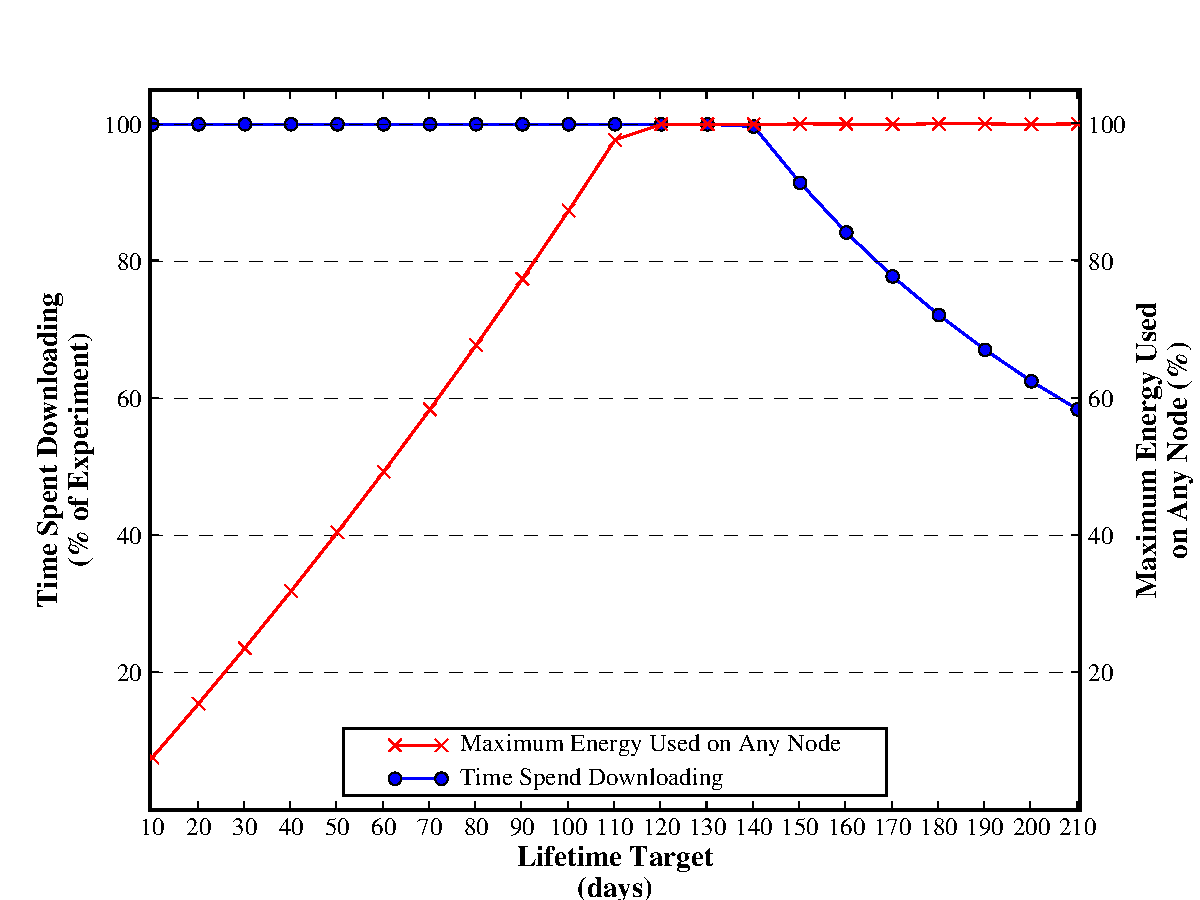
\includegraphics[width=1.0\hsize]{./figs/gwa/crossover/BANDWIDTHVENERGY.pdf}
\end{center}
\caption{\small {\bf Crossover between bandwidth and energy constraint
dominance as lifetime is varied.} 
{\em This graph shows the transition between bandwidth and energy constrained
regions for an optimal system.  The right axis shows the percent of energy
consumed by the most highly-drained node, and the left axis shows the amount
of time spent downloading.}}
\label{sec-eval-crossover}
\end{figure}



As stated in Section~\ref{sec-problem-definition}, the high-level goal of
Lance is to download a set of ADUs maximizing the total value subject to
energy and bandwidth constraints. The {\em optimal} solution is
defined as the solution to the multidimensional knapsack problem,
which yields a set of downloaded ADUs $\mathcal{O} = \{a_1, a_2, ...
a_n\}$ that maximize data value subject to bandwidth and energy
constraints. The total data value of the optimal solution 
$\hat{v}(\mathcal{O}) = \sum_{a_i \in \mathcal{O}} v_i$.
Recall that computing the optimal solution requires {\em a priori} 
knowledge of all of the ADU values sampled by the network over time.
We define {\em optimality} as the fraction of the data value 
downloaded by Lance compared to the optimal solution. That is, given
a set of downloaded ADUs $\mathcal{L}$ with total data value
$v(\mathcal{L})$, we define optimality as 
$v(\mathcal{L}) / \hat{v}(\mathcal{O})$.

%We use both simulation and
%testbed results to evaluate optimality as we vary parameters such as
%the network topology, download bandwidths, lifetime targets, 

We begin by presenting results based on a realistic system
simulator that allows us to quickly vary parameters such as 
ADU data value distribution, network topologies, download speeds,
energy costs, and target lifetimes. We also present results from 
Lance running on MoteLab~\cite{motelab}, a sensor network testbed
deployed over 3~floors of the Harvard EECS building.
Our simulation experiments use
a 10-node linear topology as well as a 25-node realistic tree topology
shown in Figure~\ref{sec-eval-topologies}(a). Both
topologies use per-node ADU download speeds based on empirical 
measurements taken using the testbed. 
In our experiments, the ADU size is 36~KB and each node samples one 
ADU every 60~seconds (or 600~bytes/s of data).

We draw ADU values from several distributions in an attempt to understand
Lance's behavior as the properties of the sampled data change.  Three value
distributions are used: uniform random, exponentially distributed, and Zipf
with exponent $\alpha = 1$.  We also make use of an ADU value distribution
based on a 6~hour seismic signal collected at Reventador Volcano, Ecuador in
2005~\cite{volcano-osdi06}.\\

The energy costs for various operations are modeled as follows.  The
background current drain of each node is set to 2~mA, based on empirical
measurements of a TMote~Sky sensor node performing high-data-rate sampling
and storing to flash.  We also measured the current consumption to download
an ADU from a sensor node, and derived the energy costs for downloading ($E_d
= 17.6$~mA/s), routing ($E_r = 16.9$~mA/s), and overhearing ($E_o = 2$~mA/s).
Our experiments assume that each node can only overhear its parent in the
routing tree; developing more detailed overhearing models is the subject of
future work.  Computing the components of the cost vector for a particular
ADU is done by multiplying the current consumption by the ADU download time
for each node either downloading, routing, or overhearing the transmission.

\subsection{Effectiveness of scoring functions}
\label{sec-eval-heuristics}

\begin{figure}[t]
\begin{small}
\begin{center}
\begin{tabular}{|l|l|ccc|}
\hline
& & \multicolumn{3}{|c|}{Scoring Functions} \\ \hline
& & Value & Cost & Cost \\
Distribution & Lifetime & Only & Total & Bottleneck \\ \hline
\multirow{3}{*}{Uniform} & 4 months & 62.4\% & 90.5\% & \textbf{93.2\%} \\
& 11 months & 43.4\% & 68.0\% & \textbf{96.9\%} \\
& 18 months & 44.6\% & 49.0\% & \textbf{90.0\%} \\ \hline
\multirow{3}{*}{Exponential} & 4 months & 83.9\% & 85.1\% & \textbf{88.0\%}
\\
& 11 months & 70.4\% & 82.0\% & \textbf{93.0\%} \\
& 18 months & 67.2\% & 72.8\% & \textbf{91.2\%} \\ \hline
\multirow{3}{*}{Zipfian} & 4 months & 84.7\% & \textbf{91.4\%} & 87.1\% \\
& 11 months & 63.8\% & 91.1\% & \textbf{96.2\%} \\
& 18 months & 53.1\% & 86.9\% & \textbf{93.8\%} \\ \hline
\end{tabular}
\end{center}
\end{small}
\caption{\small {\bf Optimality of different scoring functions.} 
{\em This table summarizes simulation results evaluating the three 
different scoring functions.  Results are shown for
several different lifetime targets and value distributions. 
{\em cost-bottleneck} out-performs the others 
in almost all cases.}}
\label{sec-eval-table}
\end{figure}

We begin by evaluating the three scoring functions described
Section~\ref{sec-lanceoptimizer}.  We want to see which is the most able to
approximate the optimal solution across a range of target lifetimes
and ADU distributions. As discussed earlier we expected
the \emph{value-only} scoring function, without considering the energy or
bandwidth overhead of downloading each ADU, to consume more 
energy downloading
high-valued ADUs when it could have increased the total data value by
downloading several slightly less-highly valued ADUs with lower costs.  The
\emph{cost-total} scoring function incorporates a notion of cost, but
will tend to favor nodes closer to the base station at the expense
of high-valued ADUs that are more routing hops away. The
\emph{cost-bottleneck} scoring function should strike a balance between 
the two, since it considers only the most significant component 
of the cost vector when ranking ADUs.

Figure~\ref{sec-eval-figlinear} shows simulation results using the 10-node
linear topology with exponentially-distributed ADU values, and a target
lifetime of 3~months.  Nodes are numbered in increasing distance from the base
station.  The graph confirms the intuition behind the scoring function
behavior.  \emph{value-only} downloads roughly equal value from each node,
but fails to match the optimal performance. \emph{cost-total} downloads more
data from nodes near the sink.  \emph{cost-bottleneck} comes close to
matching the optimal solution, retrieving over 99\% of the value retrieved by
the optimal solution.

\begin{figure}[t]
\begin{center}
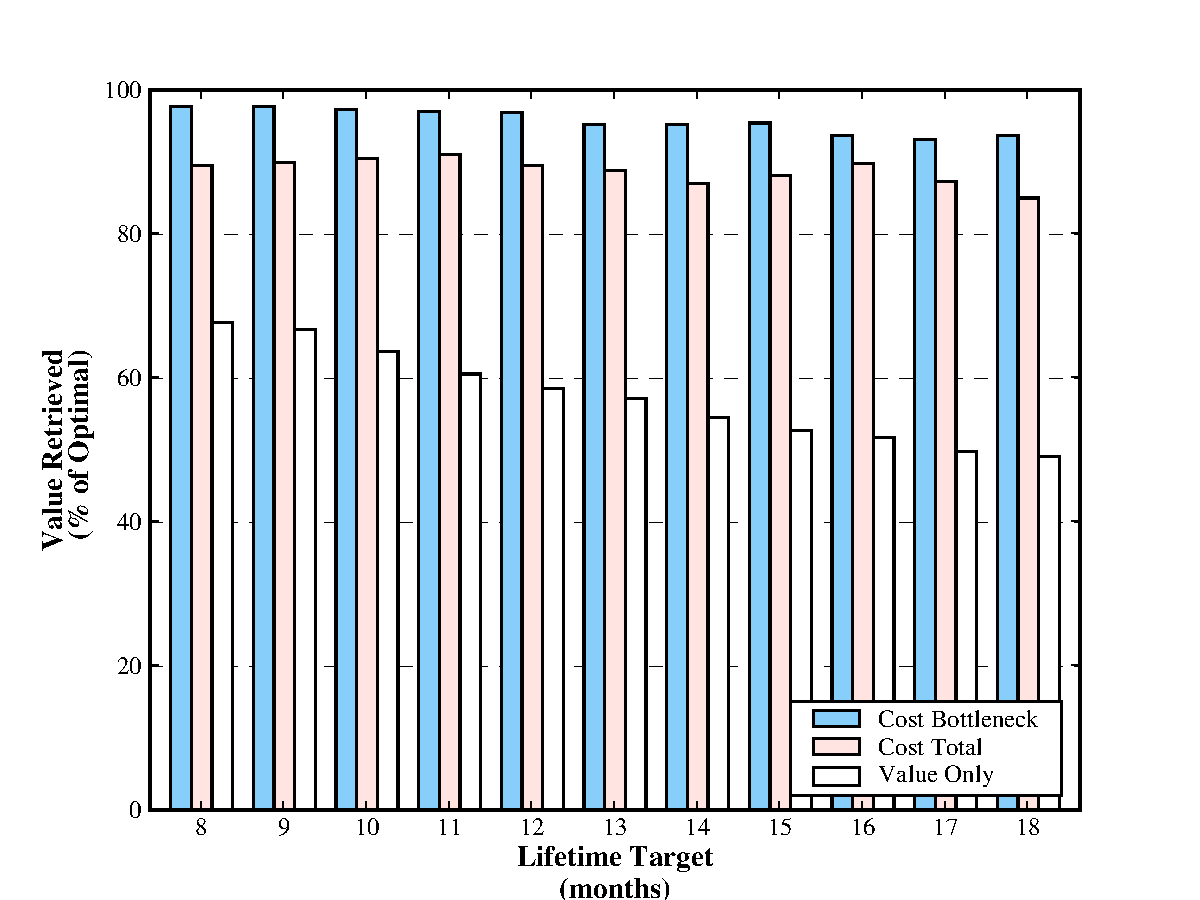
\includegraphics[width=1.0\hsize]{./figs/gwa/zipfian/POLICIES.pdf}
\end{center}
\caption{\small {\bf Scoring function performance on Zipfian distribution.}
{\em The {\em cost-bottleneck} scoring function outperforms the other two
across a range of lifetime targets.}}
\label{sec-eval-zipfian}
\end{figure}

\begin{figure}[t]
\begin{center}
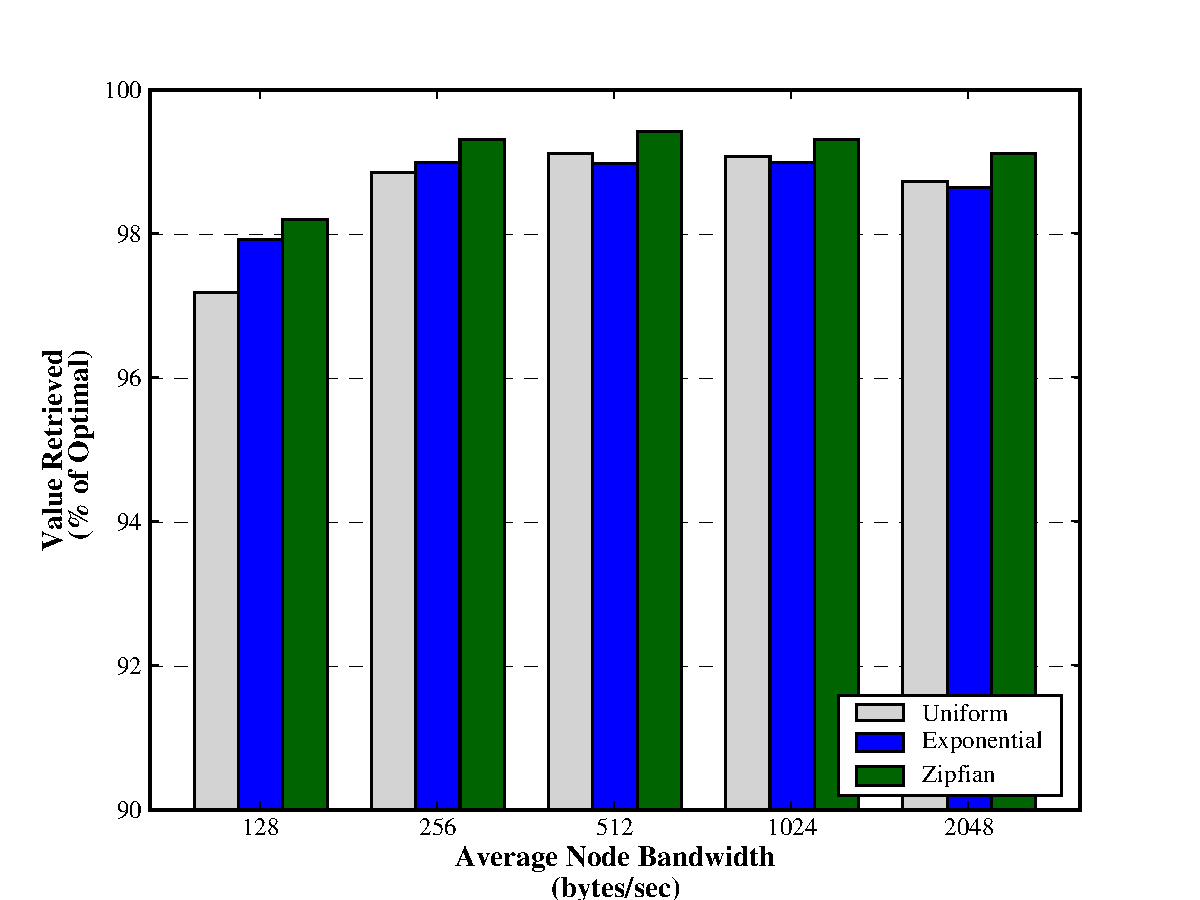
\includegraphics[width=1.0\hsize]{./figs/gwa/speeds/POLICIES.pdf}
\end{center}
\caption{\small {\bf Effect of varying download bandwidth.}
{\em Lance
maintains a high degree of optimality as the per-node download 
bandwidth is varied.
Here results are shown for the three synthetic distributions across a 25~node
tree topology and the \emph{cost-bottleneck} scoring function.  
Note that the $y$-axis starts at 90\%.}}
\label{sec-eval-figspeeds}
\end{figure}


Table~\ref{sec-eval-table} summarizes simulation results from a variety of
different lifetimes and value distributions, run on the 25-node tree
topology. The table shows that the {\em cost-bottleneck} scoring function
outperforms the other two in most cases, with optimality values
between 87.1\% and 96.9\%.
The one exception is the 4-month Zipfian data
set, where \emph{cost-total} slightly outperforms 
\emph{cost-bottleneck}. Figure~\ref{sec-eval-zipfian} shows
the effect of varying the network's target lifetime, using the 
25-node tree topology and a Zipfian data value distribution.
As the figure shows, the \emph{cost-bottleneck} scoring function 
maintains a high degree of optimality as the network bandwidth changes.

To illustrate the effect of varying lifetime targets in more detail,
Figure~\ref{sec-eval-crossover} shows how the optimal solution
transitions between bandwidth-dominant and energy-dominant constraints as the
target lifetime increases. At low lifetime targets, the system is 
bandwidth constrained and cannot download data fast enough to exhaust the 
nodes' batteries.  
At high lifetime targets, the system is energy constrained and
cannot download continuously without exhausting the nodes' batteries.  

\subsection{Bandwidth adaptation} 
\label{sec-eval-params}

Next, we evaluate the impact of varying the download bandwidth in
Figure~\ref{sec-eval-figspeeds}, using the 25-node tree topology and
the \emph{cost-bottleneck} scoring function. We vary the per-node download
bandwidth from 128~to~2048~bytes/s and peg the target lifetime at
8~months. As the figure shows, Lance performs very well
across the range of bandwidths, with optimality greater than
97\% in all cases.

\subsection{Effect of cost vector error}

Our last simulation study evaluates the effect of introducing errors into
estimated download cost. This experiment uses the 25-node topology,
\emph{cost-bottleneck} scoring function, and an exponential data
distribution.  As described in Section~\ref{sec-costassignment}, estimating
the cost of performing different operations {\em a priori} can be difficult.
As shown in Figure~\ref{sec-eval-figerror}, even a 40\% error in each
component of the cost vector $\bar{c}_i$ for a given ADU only degrades
optimality by approximately 15\%. We conclude that accurate estimations
of download costs are not strictly necessary to achieve good performance.

%%%%%%%%%%%%%%%%%%%%%%%%%%%%%%%%%%%%%%%%%%%%%%%%%%%%%%%%%%%%%%%%%%%%%%%%%

\subsection{Testbed experiments}
\label{sec-eval-policies}

\begin{figure*}[t]
\begin{center}
\begin{tabular}{cc}
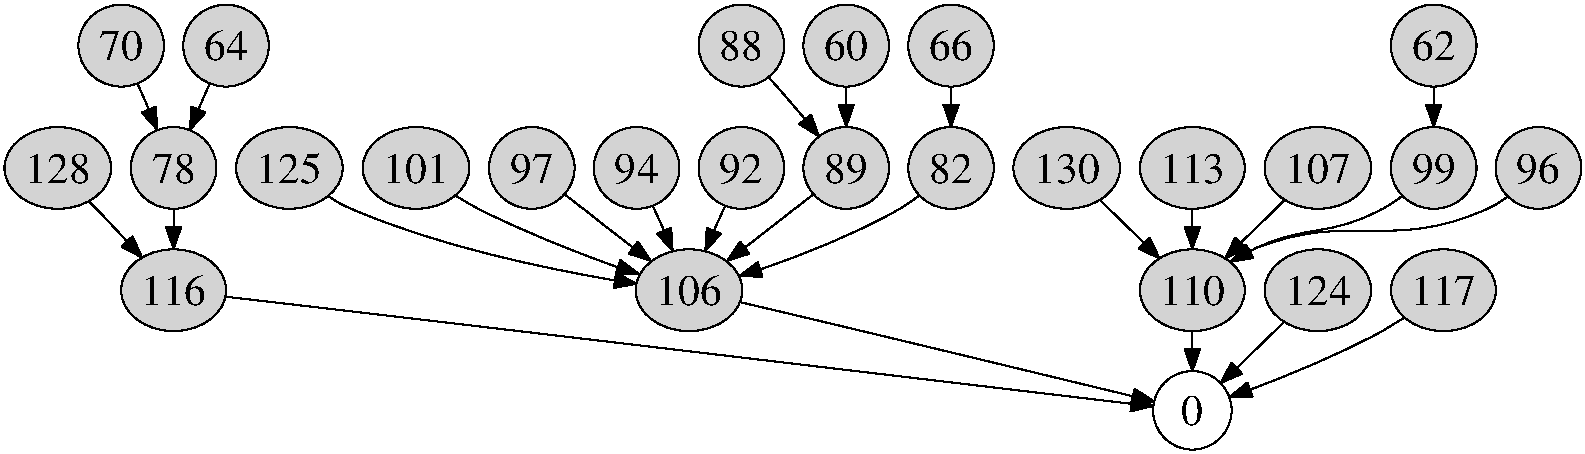
\includegraphics[width=0.45\hsize]{./figs/gwa/topologies/25.pdf} &
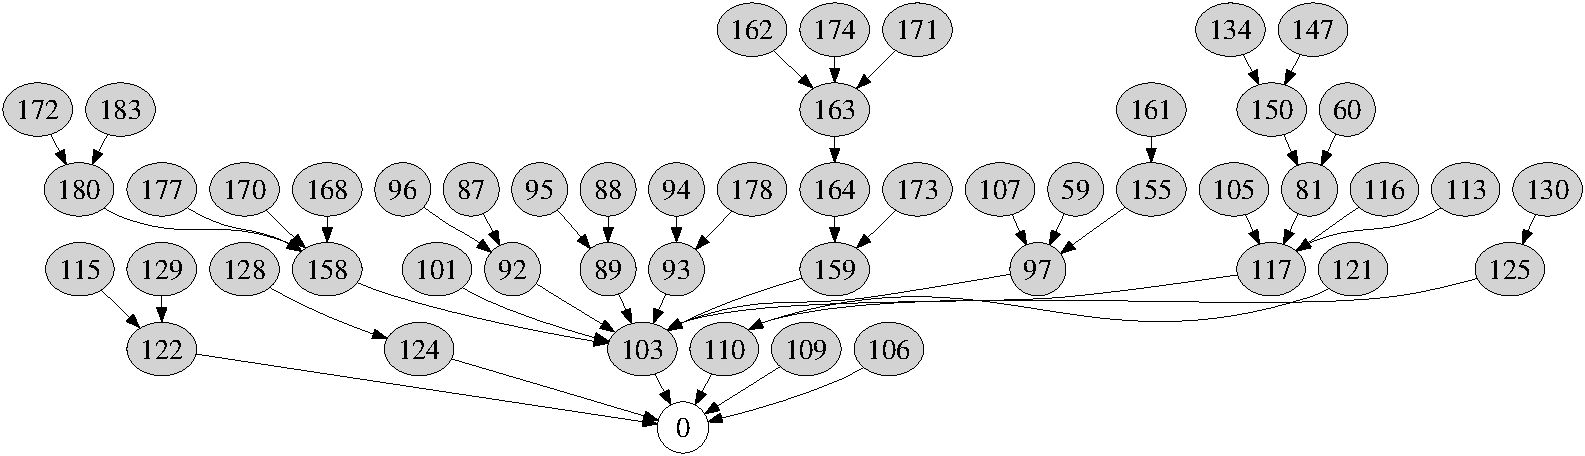
\includegraphics[width=0.45\hsize]{./figs/gwa/topologies/50.pdf} \\
(a) &
(b)\\
\end{tabular}
\end{center}
\caption{\small {\bf Topologies for testbed experiments.} 
{\em This graph shows the 25 (a) and 50 (b) node topologies used for our testbed
experiments.}}
\label{sec-eval-topologies}
\end{figure*}

\begin{figure*}[t]
\begin{center}
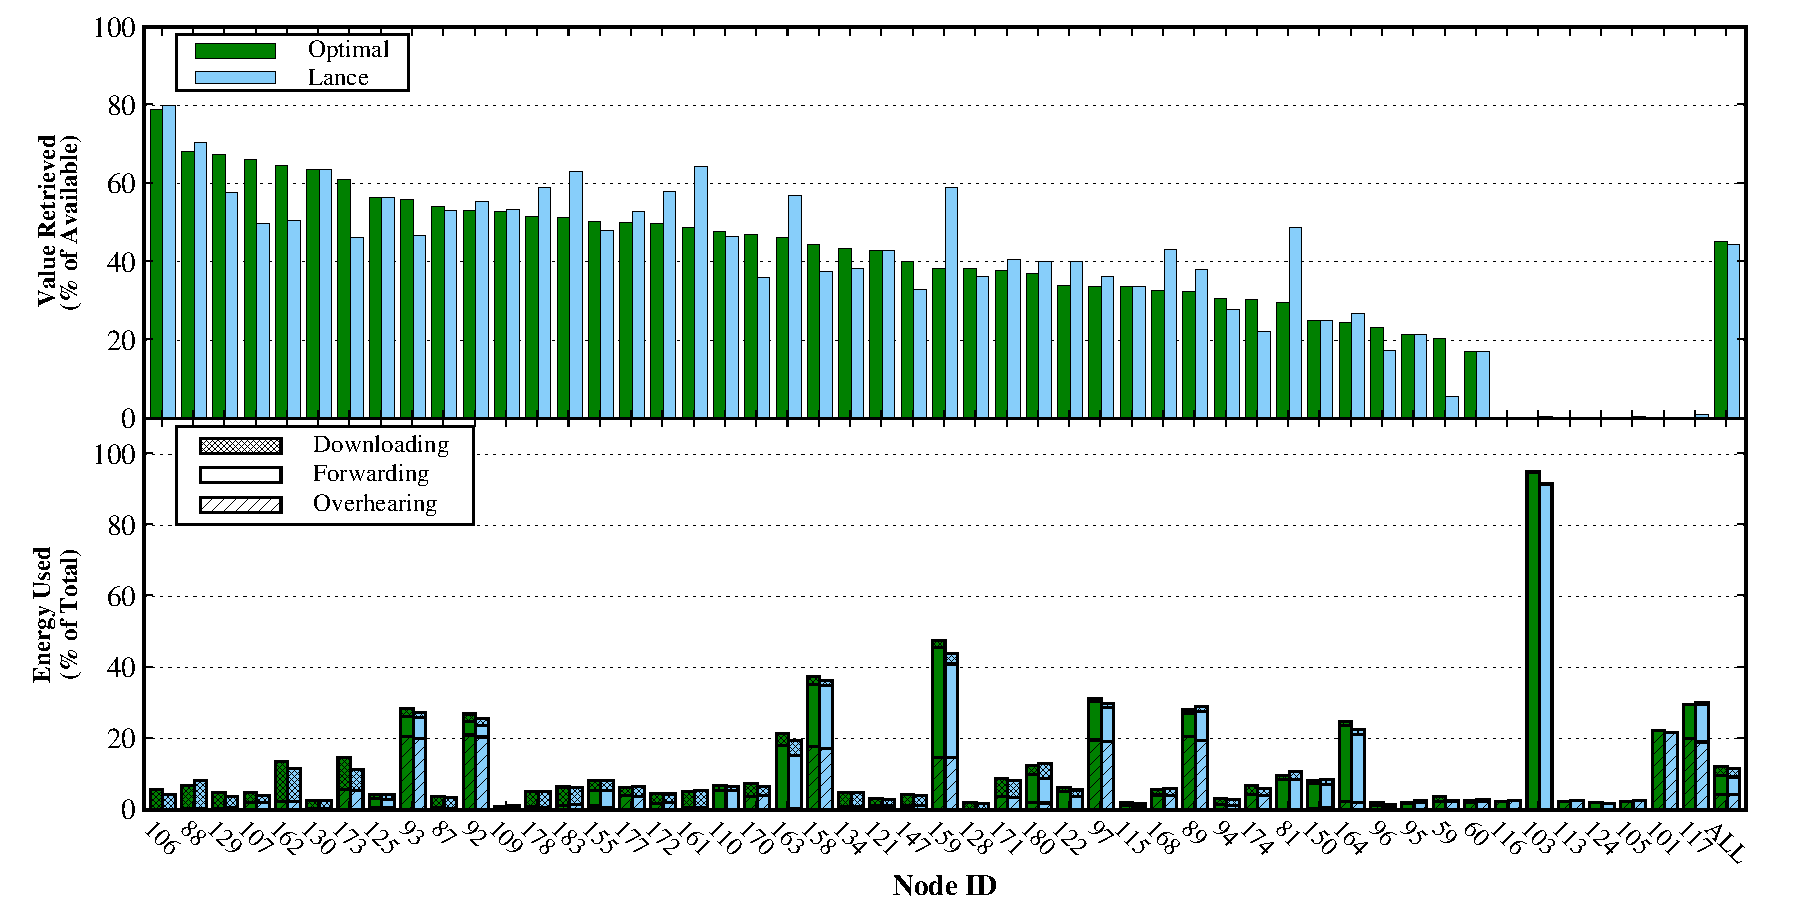
\includegraphics[width=1.0\hsize]{./figs/gwa/big/FIGURE.pdf}
\end{center}
\caption{\small {\bf Optimality and energy use in the 50-node testbed
experiment.} {\em Lance achieved near-optimal performance during 
this 8-hour testbed experiment,
retrieving 98\% of the value obtained by the offline optimal algorithm.}}
\label{sec-eval-figvolcano}
\end{figure*}

In this section, we present results from the Lance system running on the
MoteLab testbed, in 25-node and 50-node configurations shown in
Figure~\ref{sec-eval-topologies}. These experiments stress the system in a
realistic setting subject to radio interference and congestion, and exercise
the multihop routing protocol, Fetch reliable data-collection protocol, and
ADU summary traffic generated by the nodes. For these experiments, we
injected artificial ADU values directly into each node rather than relying on
the nodes sampling real sensor data; this approach allows us to perform
repeatable experiments that explore a wider range of ADU value distributions.
We use the \emph{cost-bottleneck} scoring function. 

Figure~\ref{sec-eval-figvolcano} shows the results of a 50-node testbed
experiment using a Zipfian data distribution and a target lifetime of
6~months.  The upper portion of the figure shows the amount of data value
obtained by Lance from each node, compared to the optimal solution (which was
computed offline). Nodes are sorted by decreasing optimal value. As the
figure shows, Lance achieves very close to the optimal solution, with an
optimality of 98\% overall.  In some cases, Lance incorrectly downloads more
data from some nodes and less data from others; this is due to the inherent
limitations of an online solution that cannot foresee future ADU values.  The
lower portion of the figure shows the energy breakdown for each node with
downloading, forwarding, and overhearing costs shown.  Some nodes consume
more than others because of their location in the routing tree. For example,
node~103 in uses a great deal of energy for routing packets as it is one hop
from the base station, although no ADUs are ever downloaded from that node.

\begin{figure}[t]
\begin{center}
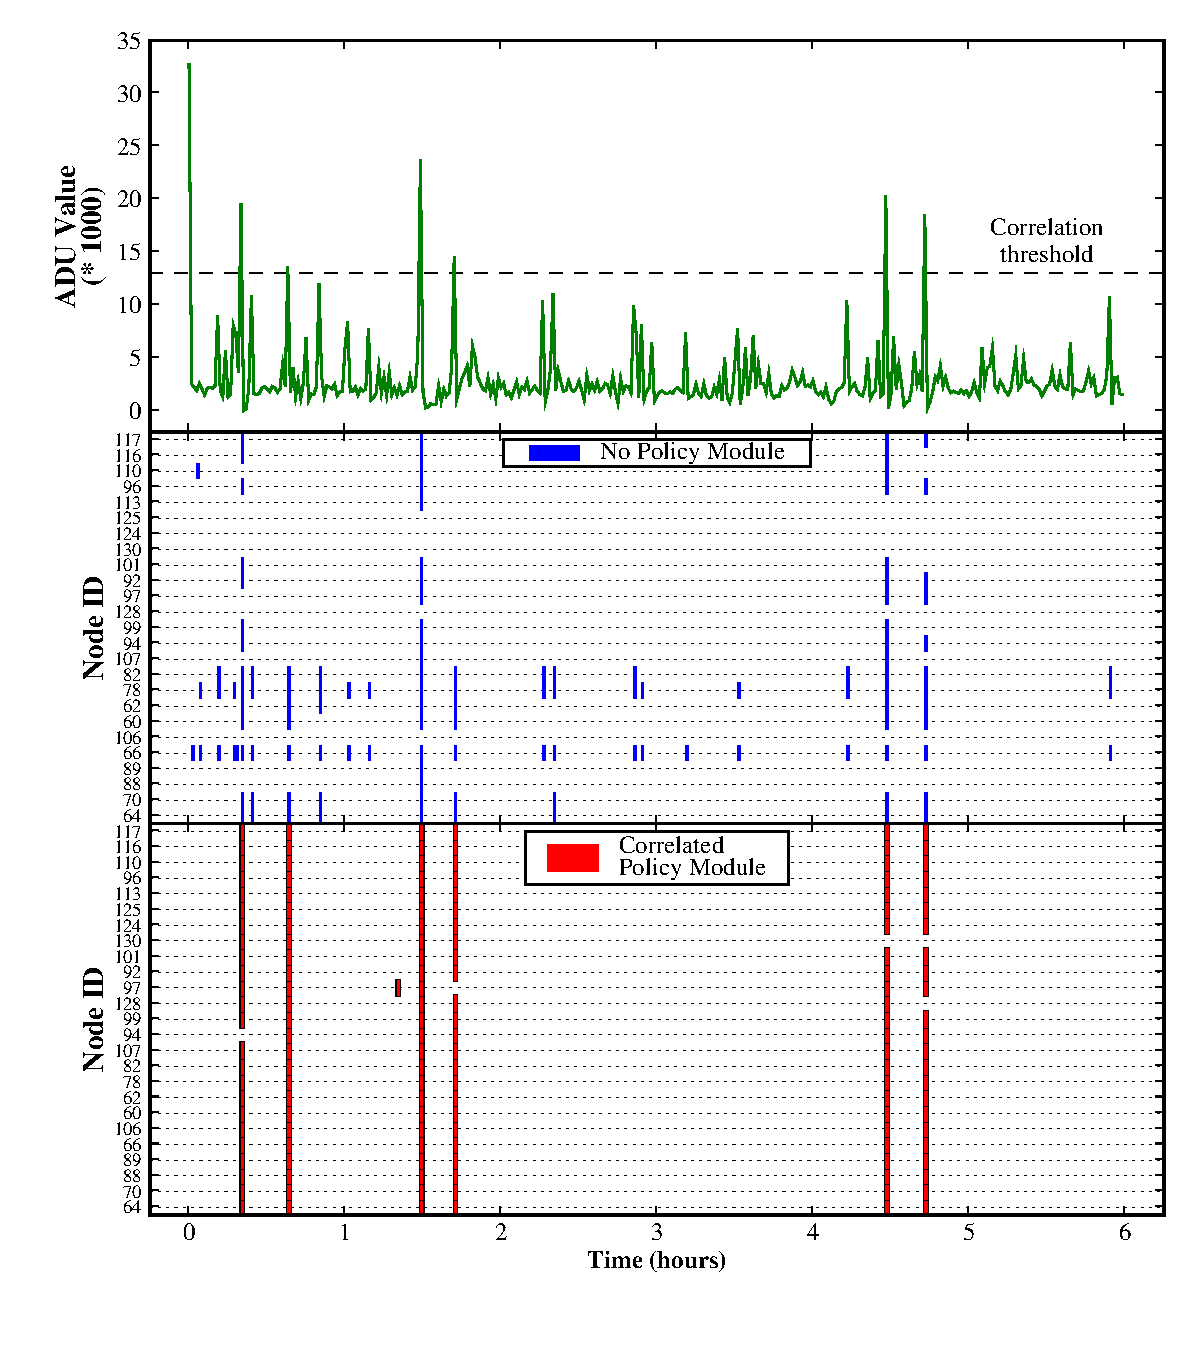
\includegraphics[width=1.0\hsize]{./figs/gwa/policy/FILL.pdf}
\end{center}
\caption{\small {\bf Usage of policy modules to affect download
distribution.} 
{\em Here we illustrate the use of policy modules in the context of
the volcano-monitoring application. The graph compares the download behavior
of the system with and without the policy module chain described in
Section~\ref{sec-ewma-deployment}, which assign greater values to ADUs
corresponding to correlated seismic activity. The graph is colored
at a particular timestamp and node ID if we downloaded that signal from that
node. The top graph shows the ADU values over time, with the threshold for
the \texttt{filter} component of the policy module chain indicated.}}
\label{sec-eval-figpolicyfill}
\end{figure}

Finally, we demonstrate the use of Lance's policy modules.  For this
experiment, we use a distribution of ADU data values based on a 6-hour
seismic trace collected at Reventador Volcano, Ecuador in
2005~\cite{volcano-osdi06}. The raw seismic data is divided into ADUs of 36
KB and ADU values $v_i$ are assigned by computing the ratio of two
EWMA~filters on the data; this assigns greater value to ADUs that contain
earthquakes, as described in Section~\ref{sec-ewma-deployment}. For each node
in the 25-node topology, the ADU values from the seismic trace are attenuated
based on a hypothetical signal source and assigned to each of the 25-nodes
based on their location with respect to the signal source. We then enable a
policy module chain, as described in Section~\ref{sec-policies}, that assigns
higher priority to ADUs that correspond to correlated seismic activity across
the network.

Figure~\ref{sec-eval-figpolicyfill} shows the result of this
experiment running on the MoteLab testbed. The upper portion of the
figure shows the ADU values over time; the middle portion, the set of ADUs
downloaded by the system with no policy modules in use; and the lower
portion, the ADUs downloaded with the policy module chain in use.
As the figure shows, the policy modules cause the network to prefer 
correlated seismic events and download an ADU from all nodes in
the network when such an event is detected. Gaps in the set of ADUs
downloaded are due to download timeouts. In one case, a single ADU 
is downloaded spuriously due to an incorrect value being reported by
that node to the base station. This use of policy modules shows the
drastic change in the system behavior that is affected without
programming the sensor nodes themselves.

%\begin{figure}[t]
%\begin{center}
%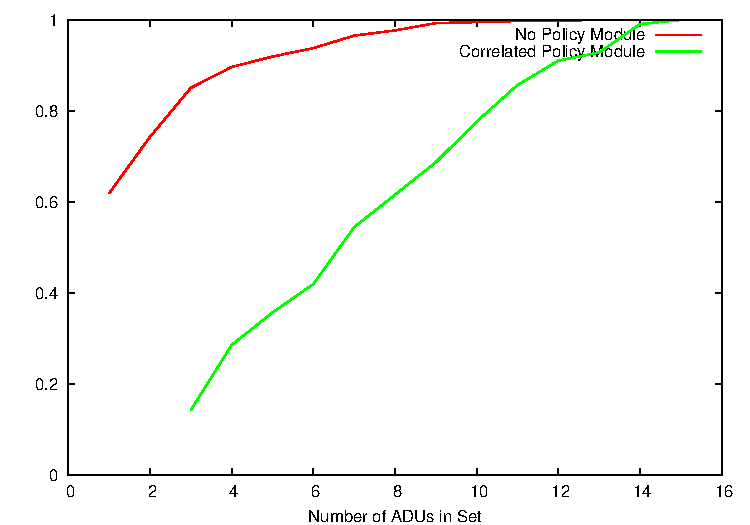
\includegraphics[width=1.0\hsize]{./figs/gwa/marm/CDF.pdf}
%\end{center}
%\caption{\small {\bf Usage of policy modules to affect download
%distribution.} 
%{\em Here we illustrate the use of policy modules in the context of
%the habitat-monitoring application. This CDF shows the distribution of the
%number of ADUs overlapping in time downloaded by our system. As can be seen,
%introducing the {\tt correlated} policy module causes Lance to download
%larger numbers of ADUs per time interval corresponding to interesting events.}}
%\label{sec-eval-figmarmot}
%\end{figure}


%\begin{figure}[t]
%\begin{center}
%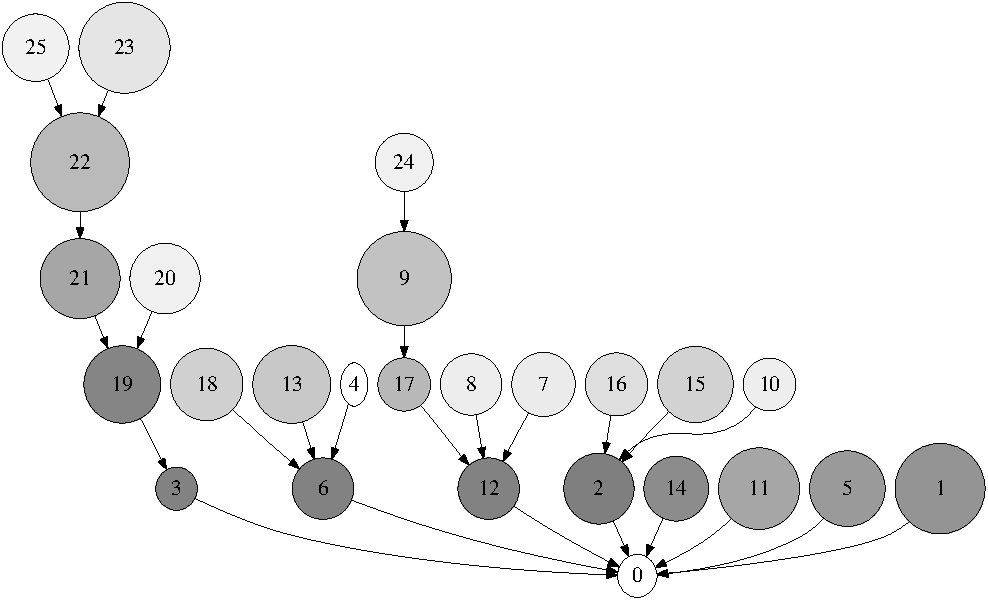
\includegraphics[width=1.0\hsize]{./figs/gwa/motelab/TOPOLOGY.pdf}
%\end{center}
%\caption{\small {\bf Topology of nodes used for the testbed experiment.} 
%{\em Sensor nodes are shaded according to the total energy consumption,
%and the size of each node represents total value of the ADUs downloaded
%from the node.}}
%\label{sec-eval-figtopology}
%\end{figure}

